\documentclass[tikz,border=10pt]{standalone}
\begin{document}
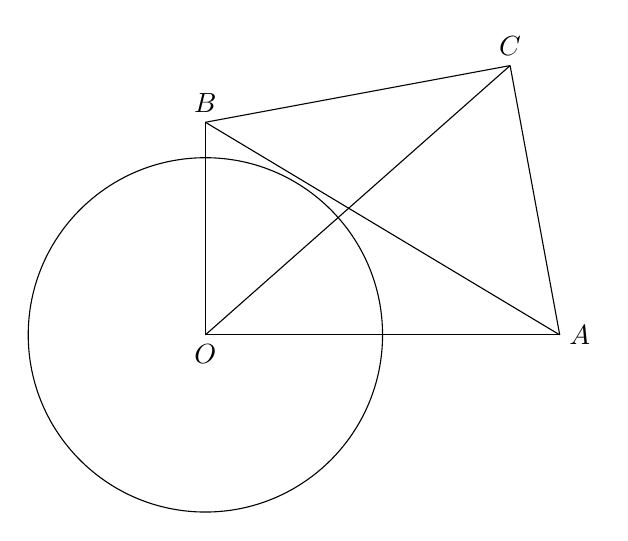
\begin{tikzpicture}[scale=0.9]
  \coordinate (O) at (0,0);
  \coordinate (B) at (0,3);
  \coordinate (A) at (5,0);
  \coordinate (C) at (4.3,3.8);

  \draw (O) circle (2.5);

  \draw (O) -- (A);
  \draw (O) -- (B);
  \draw (B) -- (A);
  \draw (B) -- (C);
  \draw (C) -- (A);
  \draw (O) -- (C);

  \node[below] at (O) {$O$};
  \node[above] at (B) {$B$};
  \node[right] at (A) {$A$};
  \node[above] at (C) {$C$};
\end{tikzpicture}
\end{document}
